% F1: testbed architecture / control-loop diagram.
% Standalone-compilable for iteration; \input{} into the paper body.
\documentclass[tikz,border=2pt]{standalone}
\usepackage{amsmath}
\usetikzlibrary{arrows.meta,positioning,fit,backgrounds}

\begin{document}
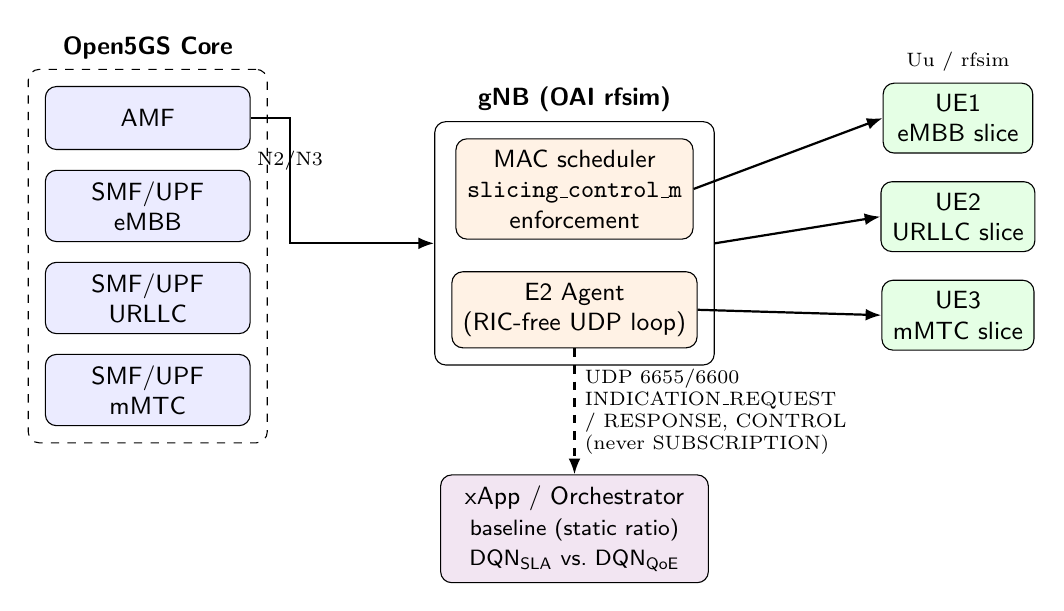
\begin{tikzpicture}[
  font=\sffamily\small,
  box/.style={draw, rounded corners, minimum height=0.8cm, align=center, inner sep=4pt},
  core/.style={box, fill=blue!8},
  gnb/.style={box, fill=orange!10},
  ue/.style={box, fill=green!10, minimum width=1.9cm},
  xapp/.style={box, fill=violet!10},
  arrow/.style={-{Latex[length=2mm]}, thick},
  dashedarrow/.style={-{Latex[length=2mm]}, thick, dashed},
]

% -- Core --
\node[core, minimum width=2.6cm] (amf) {AMF};
\node[core, minimum width=2.6cm, below=0.25cm of amf] (smf1) {SMF/UPF\\eMBB};
\node[core, minimum width=2.6cm, below=0.25cm of smf1] (smf2) {SMF/UPF\\URLLC};
\node[core, minimum width=2.6cm, below=0.25cm of smf2] (smf3) {SMF/UPF\\mMTC};
\node[draw, dashed, rounded corners, fit=(amf)(smf1)(smf2)(smf3), inner sep=6pt, label={[font=\sffamily\bfseries\small]above:Open5GS Core}] (core) {};

% -- gNB --
\node[gnb, minimum width=3.0cm, right=2.6cm of smf1.north east, anchor=north west, yshift=0.4cm] (mac) {MAC scheduler\\\texttt{slicing\_control\_m}\\enforcement};
\node[gnb, minimum width=3.0cm, below=0.4cm of mac] (e2) {E2 Agent\\(RIC-free UDP loop)};
\node[draw, rounded corners, fit=(mac)(e2), inner sep=6pt, label={[font=\sffamily\bfseries\small]above:gNB (OAI rfsim)}] (gnbbox) {};

% -- UEs --
\node[ue, right=2.4cm of mac, yshift=0.9cm] (ue1) {UE1\\eMBB slice};
\node[ue, below=0.35cm of ue1] (ue2) {UE2\\URLLC slice};
\node[ue, below=0.35cm of ue2] (ue3) {UE3\\mMTC slice};

% -- xApp / arms --
\node[xapp, minimum width=3.4cm, below=1.6cm of e2] (xapp) {xApp / Orchestrator\\\footnotesize baseline (static ratio) \\ \footnotesize DQN$_{\text{SLA}}$ vs.\ DQN$_{\text{QoE}}$};

% -- Connections --
\draw[arrow] (amf.east) -- ++(0.5,0) coordinate (n2n3) -- (n2n3 |- gnbbox.west) node[midway, above, font=\scriptsize] {N2/N3} -- (gnbbox.west);

\draw[arrow] (mac.east) -- (ue1.west);
\draw[arrow] (gnbbox.east) -- (ue2.west);
\draw[arrow] (e2.east) -- (ue3.west);
\node[font=\scriptsize, above=0.02cm of ue1] {Uu / rfsim};

\draw[dashedarrow] (e2.south) .. controls +(0,-1) and +(0,1) .. node[right, font=\scriptsize, align=left] {UDP 6655/6600\\INDICATION\_REQUEST\\ / RESPONSE, CONTROL\\(never SUBSCRIPTION)} (xapp.north);

\end{tikzpicture}
\end{document}
